\section{Section 1}
\begin{frame}[c]{Test Frame} % 参数c表示内容垂直居中,默认是顶部对齐[t]
    Reference here \cite{Cheplygina2018NotsosupervisedAS}
    
    这是一段中文测试
    formula:
    \[Dice = \frac{2 |A \cap B|}{|A| + |B|}\]
\end{frame}
 
\section{Section 2}
\begin{frame}[c]{Frame Title}
    \begin{columns}
    \column{0.5\textwidth}
    This is a text in first column.
    $$E=mc^2$$
    \begin{itemize}
    \item First item
    \item Second item
    \end{itemize}
     
    \column{0.5\textwidth}
    This text will be in the second column
    and on a second tought this is a nice looking
    layout in some cases.
    \end{columns}
\end{frame}


\begin{frame}{Frame Title}

\begin{columns}
\column{0.5\textwidth}
\begin{figure}
    \centering
    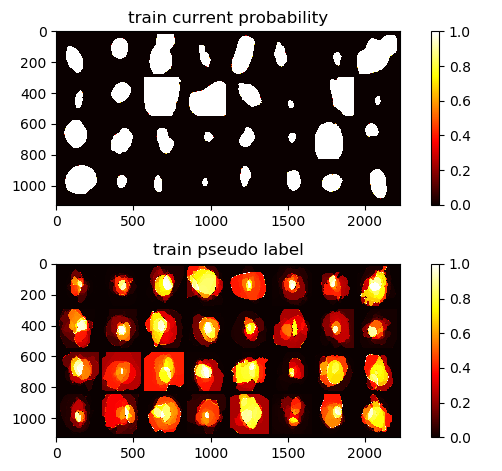
\includegraphics[width=1.\textwidth]{images/before.png}
    \caption*{Before}
\end{figure}

\column{0.5\textwidth}
\begin{figure}
    \centering
    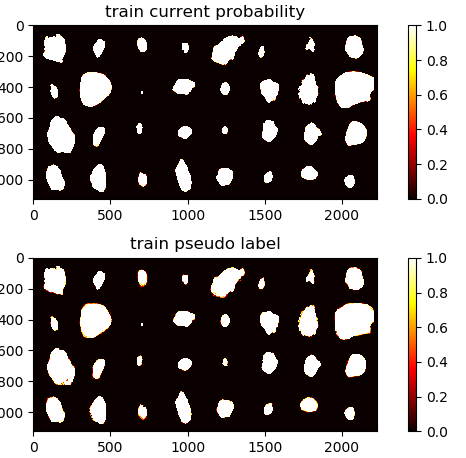
\includegraphics[width=1.\textwidth]{images/after.png}
    \caption*{After}
\end{figure}
\end{columns}
\end{frame}

\subsection{subsection 1}